\documentclass[a4paper,12pt,english]{article}
\usepackage[a4paper]{geometry}
\usepackage[english]{babel}
\usepackage{verbatim}
\usepackage{minted}
\usepackage[utf8]{inputenc}
\usepackage{graphicx}
\usepackage{float}
\usepackage{caption}
\usepackage{ mathrsfs }
\title{\textbf{Under Actuated Robotics - Workshop 1}}
\author{Stefan Ravn van Overeem – stvan13@student.sdu.dk}

\begin{document}
\maketitle
\newpage
\section{Equations of motion}
I'm going to derive the equations of motion of a system consisting of a pendulum with a moving mass hanging from a spring using the Lagrange equation. The system can be seen on figure 1.
		\begin{figure}[H]
			\centering
			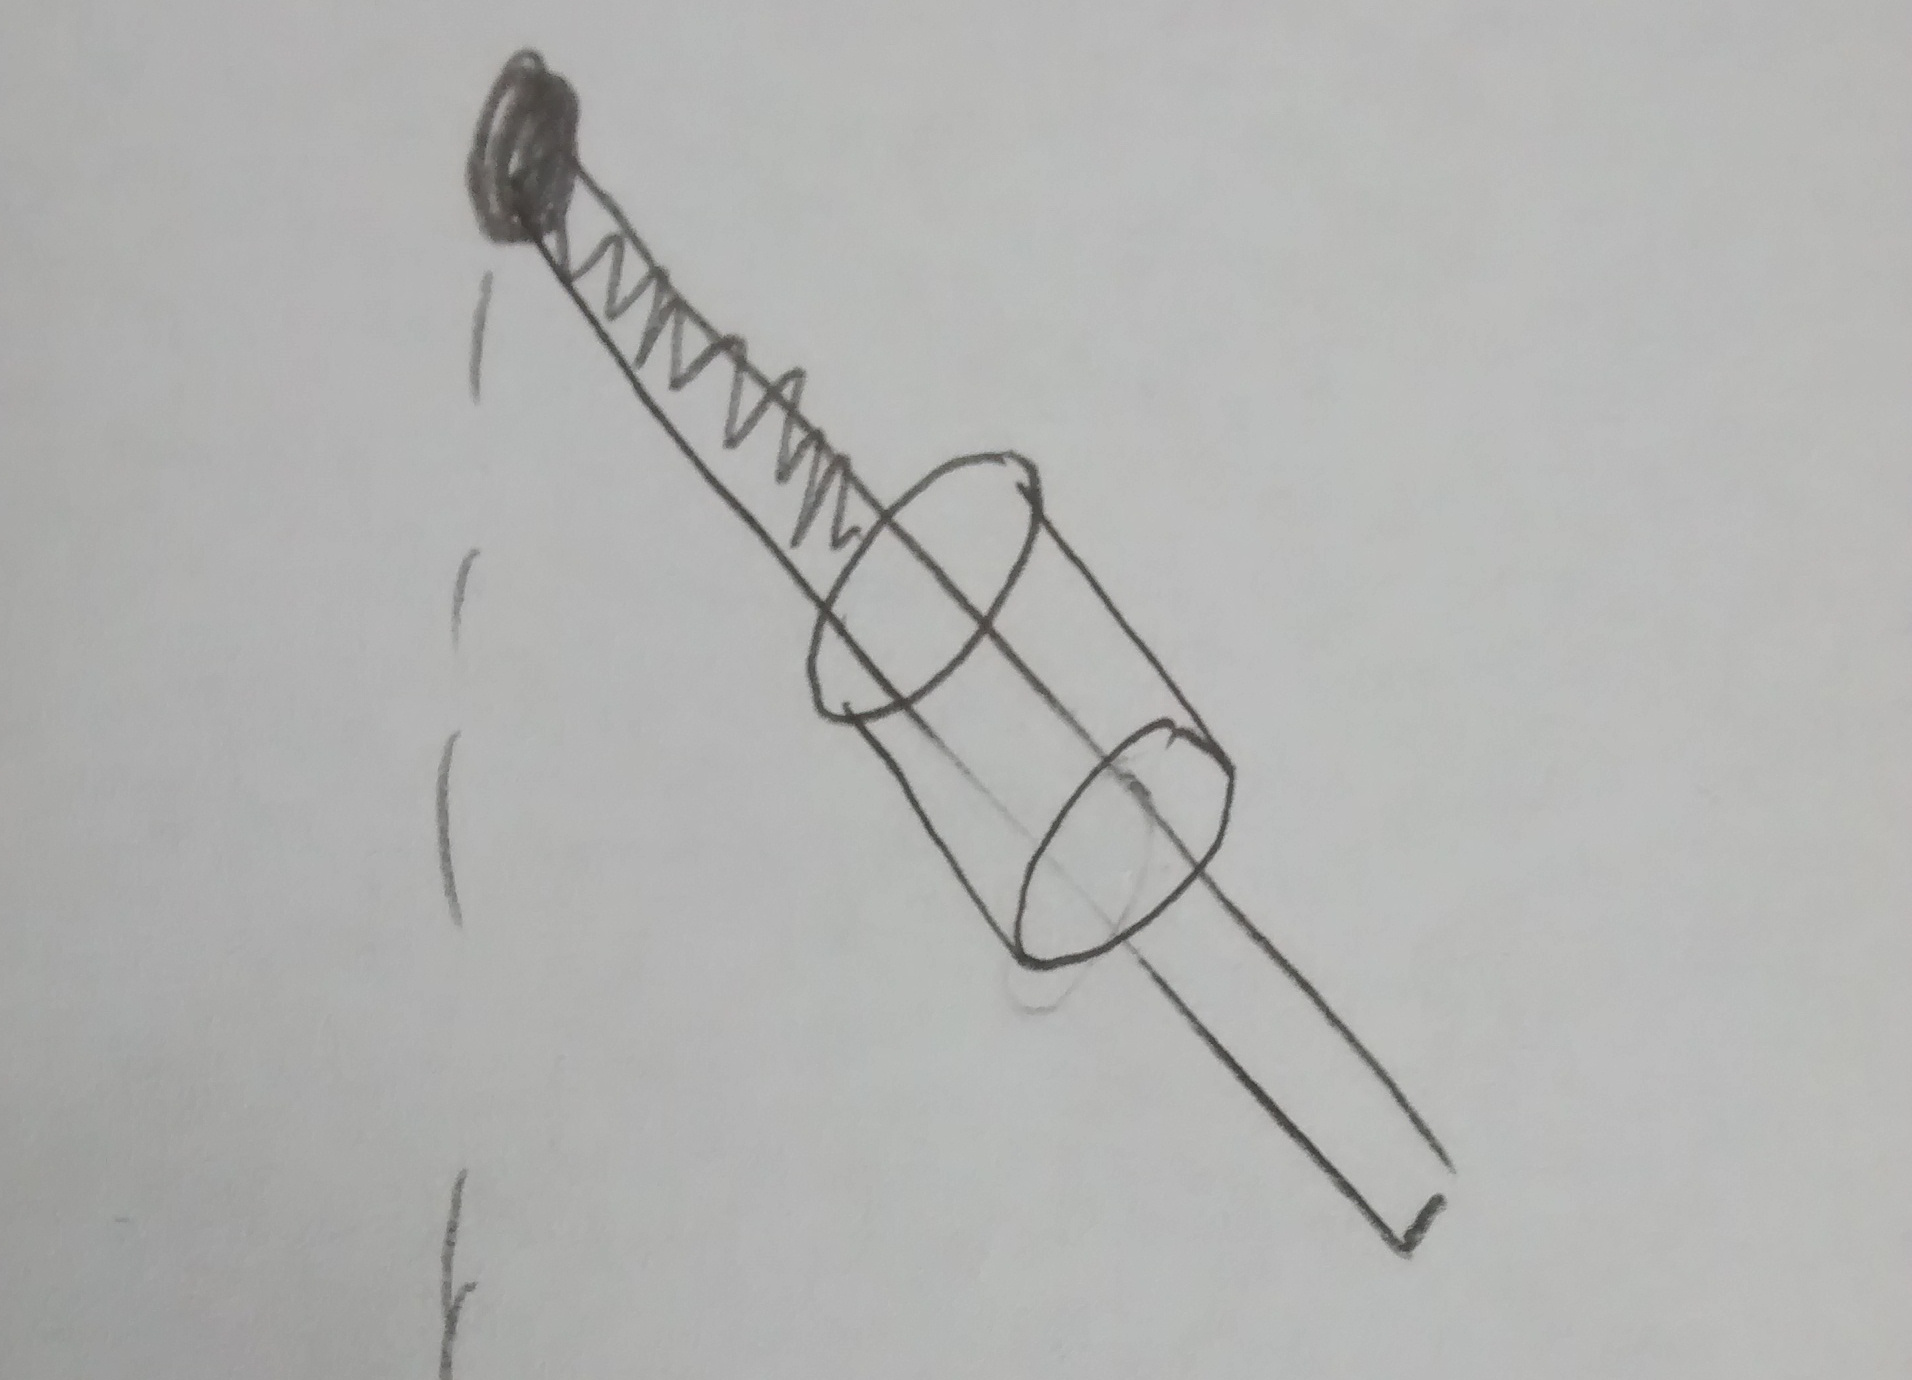
\includegraphics[scale=0.13]{system.jpg}
			\caption{}
		\end{figure}

First we must decide on some generalised coordinates. Here, we choose the angle of the pendulum, $\theta$, and the distance down the rod, that the moving mass is. They can be seen on figure 2.
		\begin{figure}[H]
			\centering
			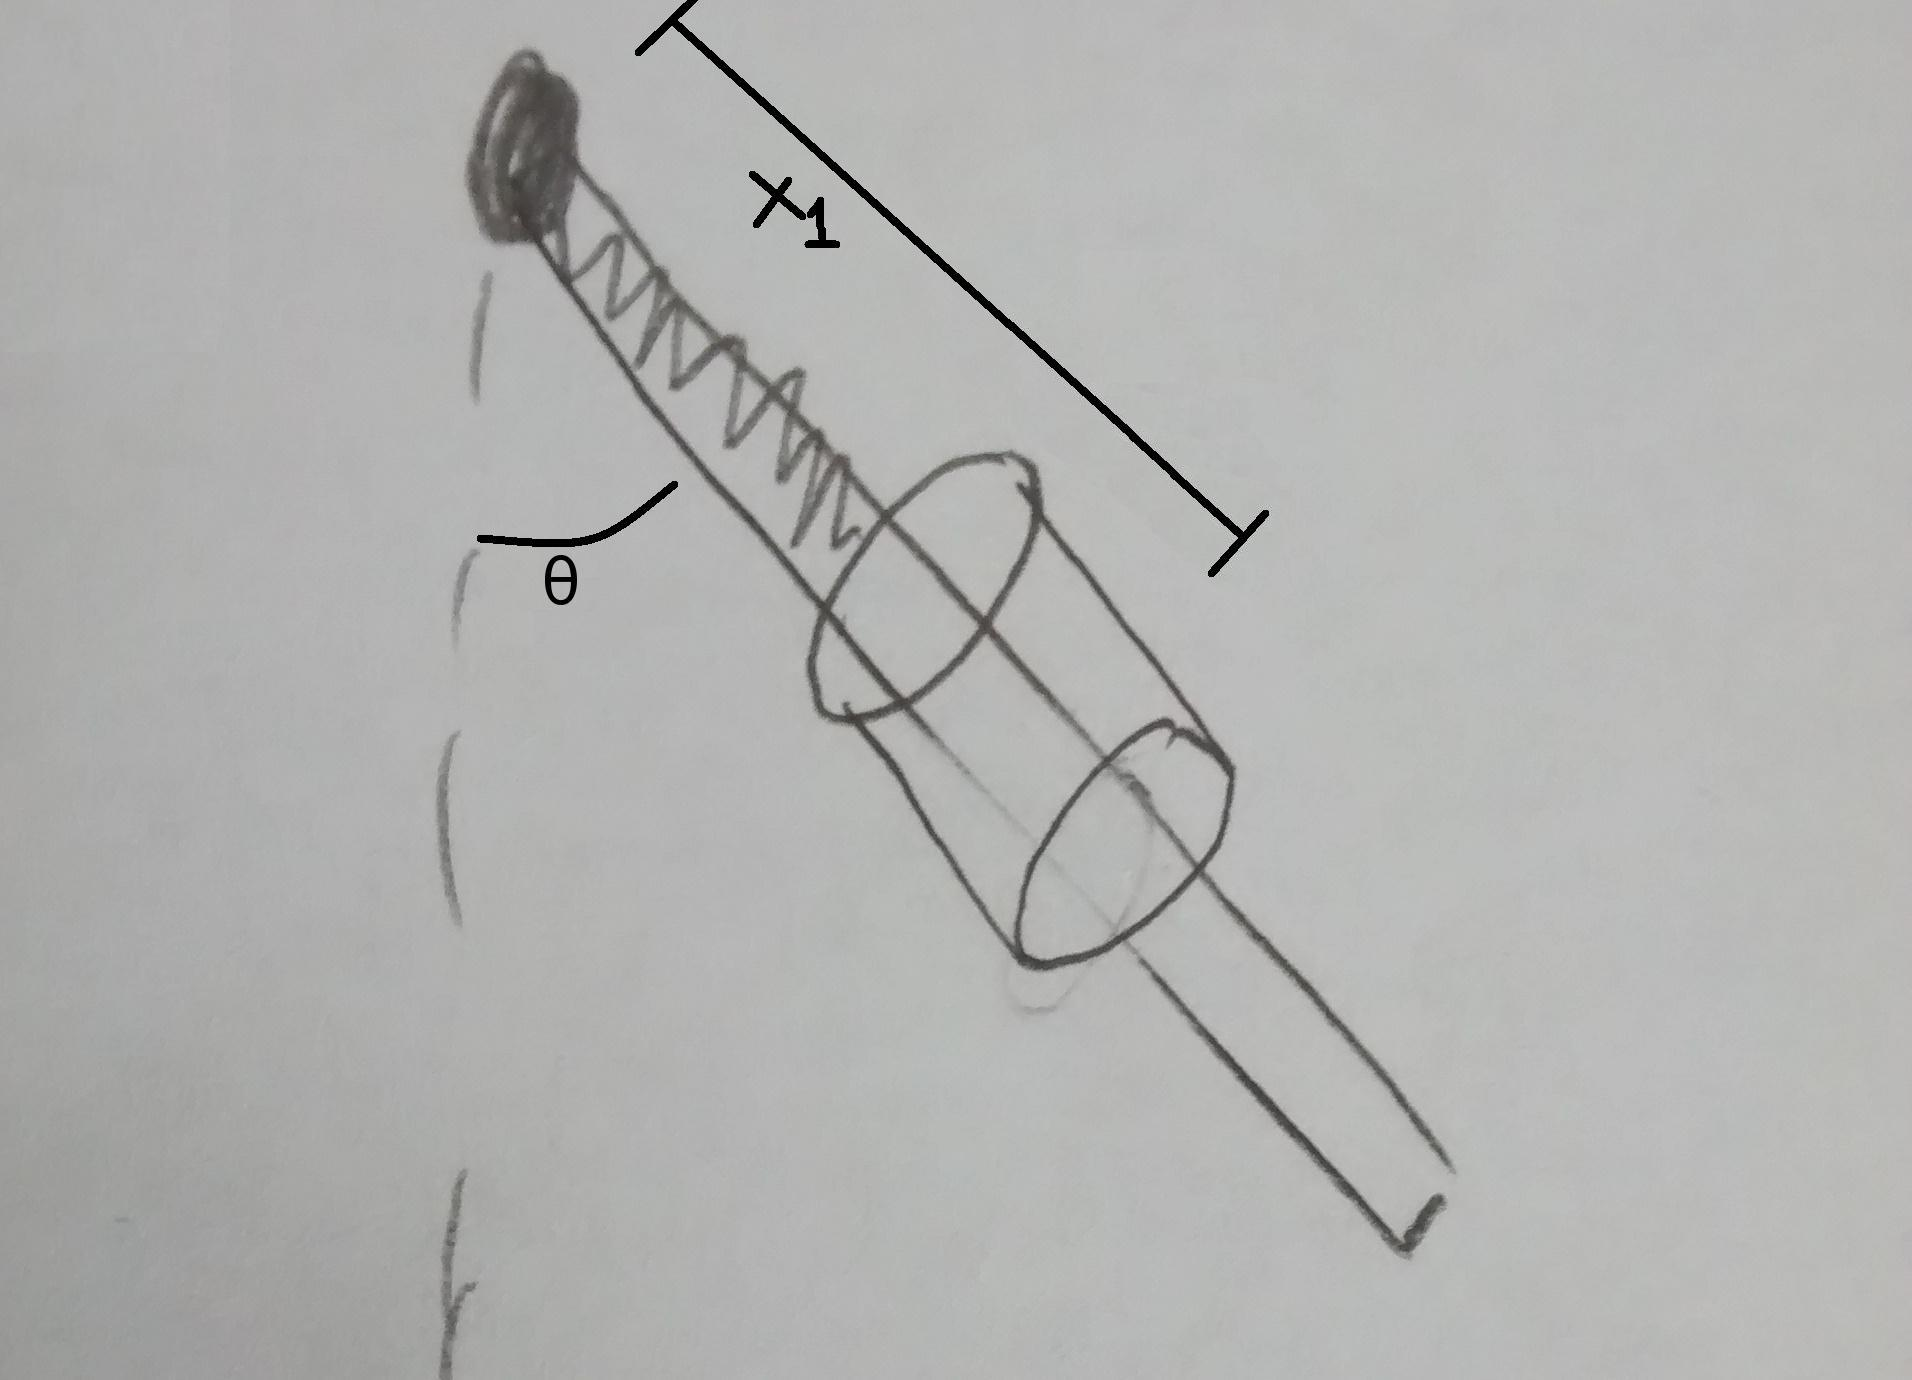
\includegraphics[scale=0.13]{systemcoordinates.jpg}
			\caption{}
		\end{figure}
The coordinates are independent, as we can lock one, and the other can still move, and they are complete, as they completely describe the state of the system. Also, they are holonomic, as there is as many degress of freedom, as coordinates.
Thus, we can apply the lagrange equation:
$$\mathscr{L} = T - V$$
Where T is the kinetic energy and V is the potential energy.

We must define some properties of the system. The rod have the following properties:
\begin{itemize}
	\item $M_1$, the mass of the rod.
	\item $I_{zz1}$, its moment of inertia around the point where it swing, which we will call A.
	\item $L_1$ the lenght of the rod.
	\item $G_1$, it's center of mass = $\frac{L_1}{2}$.
\end{itemize}



The sleeve have the following properties:
\begin{itemize}
	\item $M_2$, the mass of the sleeve.
	\item $G_2$, the center of mass.
	\item $I_{zz2}$, its moment of inertia around $G_2$.
	\item $L_2$ the lenght of the sleeve.
\end{itemize}

furthermore, the spring also have a spring cooeficient K, and an unstretched lenght, $L_0$.


Now, we start writing the equation for potential energy.

The potential energy stored in the spring is:
$$V_{spring} = \frac{1}{2} \cdot K \left (x_1 - L_0 - \frac{L_2}{2} \right)^2$$

The potential energy stored in the rod due to gravity:

$$V_{Rod} =  M_1 \cdot g \cdot \frac{L_1}{2} \cdot \left (1 - cos (\theta) \right )$$

The potential energy stored in the sleeve due to gravity:

$$V_{Rod} =  M_2 \cdot g \cdot \left( L_0 + \frac{L_2}{2} \right) - M_2 \cdot g \cdot x_1 \cdot cos(\theta) $$

Thus, in total we get:

$$V= \frac{1}{2} \cdot K \left (x_1 - L_0 - \frac{L_2}{2} \right)^2 + M_1 \cdot g \cdot \frac{L_1}{2} \cdot \left (1 - cos (\theta) \right ) +  M_2 \cdot g \cdot \left( L_0 + \frac{L_2}{2} \right) - M_2 \cdot g \cdot x_1 \cdot cos(\theta)$$

Now, we write the equation for kinetic energy.

$$T = \left ( \frac{1}{2} \cdot I_{zz1} + \frac{1}{2} \cdot  I_{zz2}   \right) \cdot \dot{\theta}^2 + \frac{1}{2} \cdot M_2 \cdot \left( \dot{x_1}^2 + x_1^2 \cdot \dot{\theta}^2 \right )$$ 

Now we have the equations, and can apply lagrange to it.
The lagrange equation says:
$$\frac{d}{d t} \frac{\partial T}{\partial \dot{q}_j} - \frac{\partial T}{\partial q_j} + \frac{\partial V}{\partial q_j} = Q_j$$

As we in this system says, that we have no external force, it becomes:

$$\frac{d}{d t} \frac{\partial T}{\partial \dot{q}_j} - \frac{\partial T}{\partial q_j} + \frac{\partial V}{\partial q_j} = 0$$

We number the terms 1, 2, 3 for convenience.

We have to apply lagrange for each generalised coordinate. 

We start with $x_1$:

\begin{itemize}
\item 1: $\frac{d}{d t} \left ( \frac{\partial T}{\partial \dot{x_1}} \right ) = M_2 \cdot \ddot{x_1}$
\item 2: $- \frac{\partial T}{\partial x_1} = - M_2 \cdot x_1 \cdot \dot{\theta}^2 $
\item 3: $\frac{\partial V}{\partial x_1} = K \left(x_1 - L_0 - \frac{L_2}{2} \right) - M_2 \cdot g \cdot cos(\theta)  $
\end{itemize}
We put them all together and get
$$ M_2 \cdot \ddot{x_1} - M_2 \cdot x_1 \cdot \dot{\theta}^2 + K \left(x_1 - L_0 - \frac{L_2}{2} \right) - M_2 \cdot g \cdot cos(\theta) = 0$$

We now do the same with $\theta$:

\begin{itemize}
\item 1: $\frac{d}{d t} \left ( \frac{\partial T}{\partial \dot{\theta}} \right ) = \left( I_{zz1} + I_{zz2} + M_2 \cdot x_1^2 \right) \cdot \ddot{\theta} + 2 \cdot M_2 \cdot x_1 \cdot \dot{x_1} \cdot \dot{\theta}$
\item 2: $- \frac{\partial T}{\partial \theta} = 0  $
\item 3: $\frac{\partial V}{\partial \theta} =  M_2 \cdot g \cdot x_1 \cdot sin(\theta) + M_1 \cdot g \cdot \frac{L_1}{2} \cdot sin(\theta)$
\end{itemize}
We put them all together and get
$$ \left( I_{zz1} + I_{zz2} + M_2 \cdot x_1^2 \right) \cdot \ddot{\theta} + 2 \cdot M_2 \cdot x_1 \cdot \dot{x_1} \cdot \dot{\theta} +  M_2 \cdot g \cdot x_1 \cdot sin(\theta) + M_1 \cdot g \cdot \frac{L_1}{2} \cdot sin(\theta) = 0$$

Now, to implement this in a simulation, we need to have expressions for $\ddot{x_1}$ and $\ddot{\theta}$.

Thus, we isolate them.
$$\ddot{x_1} = x_1 \cdot \dot{\theta}^2 - \frac{K \cdot (x_1 - L_0 - \frac{L_2}{2})}{M_2} + g \cdot cos(\theta)$$


$$\ddot{\theta} = \frac{M_2 \cdot x_1 \cdot (-2 \cdot \dot{x_1} \cdot \dot{\theta} - g \cdot sin(\theta)) - M_1 \cdot g \cdot \frac{L_1}{2} \cdot sin(\theta)}{I_{zz1} + I_{zz2} + M_2 \cdot x_1}$$

Now we are ready to implement the simulation.
\end{document}
